
%***********************************************************************

% This is a template to be used for the preparation of
% papers submitted to the 30th International Workshop on
% Statistical Modelling, to be held in Linz, Austria,
% July 6-10, 2015.

% Please follow the following general guidelines:
%
% (1) Do not specify any definitions, commands or style parameters.
%     Upon submission, your file will be checked for presence of
%     \newcommand or \def statements and if found, error message will be reported
%     by the submission form.
%
% (2) Follow the template below very tightly.
%
% (3) Include .pdf figures using the \includegraphics
%      command, an example of which are given below.
%
% (4) Use file names which begin with the surname of the first author.
%
% (5) When creating labels for cross-references, please start always
%     by surname of the first author, e.g., \label{smith:likelihood}
%
% (6) The template below contains some example materials
%      to guide you through the preparation of your paper.  However,
%      remove all the redundant material from your final document
%      before submitting.

% The guidelines above are needed in order to be able to combine all
% the papers into a single proceedings book of acceptable quality.
% Please follow the guidelines as strictly as possible. Deviations may
% result in papers being either refused by the registration form
% or sent back to the authors with the request to change
% their documents according to the guidelines.

% Special characters:
% Please do not use special characters (e.g., accents).
% Use TeX composition instead, such as \~n, \'a, \`e, \v{s}, \r{u} etc.

% Changes as of IWSM 2013:
%  * \usepackage{booktabs} added which allows \toprule et al. in the tabular environment
%    (\hline\hline is not longer used)
%  * '^\T' added in iwsm.sty to denote transposed vectors and matrices within math (see example below)
%  * \usepackage{amsmath, amssymb} introduced since IWSM 2012 is allowed (allowing usage of boldsymbols
%    and other handy constructions (align, pmatrix etc.) within math)
%  * \usepackage{psfrag} introduced since IWSM 2012 is NOT allowed
%
%

%***********************************************************************
% PLEASE LEAVE THIS PART UNCHANGED
%***********************************************************************

\documentclass[twoside]{report}
\usepackage{iwsm}
\usepackage{graphicx}
\usepackage{amsmath, amssymb}
\usepackage{booktabs}

% Please do not specify any new definitions, any new commands,
% and do not specify any style parameters.
% The preamble of the document should be left unchanged.

\begin{document}

%***********************************************************************
% PLEASE INSERT YOUR CONTENT FROM HERE
%***********************************************************************

% Title and running title to be used as left header:
\title{Exploring LD decay with quantiles -- a case study}
\titlerunning{Quantiles for LD decay}

% Authors and running list of authors to be used as right header:
\author{Federico Torretta\inst{1}, Sabine K. Schnabel\inst{2}, Matthias Westhues\inst{3}}
\authorrunning{Torretta et al.}    %% use \authorrunning{Surname 1} if only 1 author
                                    %% use \authorrunning{Surname 1 and Surname2} if two authors
                                    %% use \authorrunning{Surname 1 et al.} if more than two authors

% Institutes of all authors
% Include city and country of each institute, do not include the full address.
\institute{Universit\`a di Palermo, Italy \and Biometris, Wageningen University and Research Centre,
The Netherlands \and Universit\"at Hohenheim, Germany}

% E-mail of presenting author for correspondence
\email{sabine.schnabel@wur.nl}

% Brief abstract of the paper:
\abstract{Abstract text}

% Keywords (at most 5):
\keywords{Keyword1; Keyword2; Keyword3.}

% Produce the title:
\maketitle

%***********************************************************************

% Sections and subsections (do not use lower levels):

\section{Introduction and motivation}

\begin{itemize}
\item Decreasing costs of genotyping $\rightarrow$ data readily available 
\item More markers $\rightarrow$ more information about genetic structure available
\item More data available does not forcedly result in more information available. The sheer 
	amount of data 
	(Stichwort BIG DATA) might be a problem to deal commonly encountered. Even exploration is 
	a challenge.
\item manage $\rightarrow$ explore $\rightarrow$ analyse
\item Here we focus on exploring/quantifying LD decay.
\item As an exploratory tool we will be using quantile regression (general references).
\item Data: (local) LD decay in Maize
\end{itemize}






%Text for the first section. This section will have two subsections.
%
%The hat matrix is defined as
%$$
%H=X(X^\T X)^{-1}X^\T
%$$
%Please note we use \verb|^\T| to mean transposed matrices and vectors.
%
%\subsection{Section 1.1}
%Text for the first subsection within section 1. (Do you really need subsections ?)


\section{Section 2}
Text for the second section. This section will have no subsections.



%***********************************************************************

% Tables can be included at any place in the text.
% As general format, use tables with horizontal lines only
% (i.e., no vertical lines separating columns).
% Start and end each table with a double horizontal line.
% Tables are incorporated using a table environment:

\begin{table}[!hb]\centering
% A caption is put above the table and a label is defined
% to be used for reference to this specific table.
% Use labels which are very unlikely to be used by
% other contributors; for example, use labels starting
% with the surname of the first author.
\caption{\label{smith:tab1} Caption text \textbf{ABOVE} the table.}
% A table with three columns, where the first is left aligned,
% the second has centred entries, and the third is right aligned,
% is generated as follows (note: if requested, use \cmidrule{} instead of \cline{})
\medskip
\begin{tabular}{lcr}
% First line:
\toprule[0.09 em]
% The body of the table:
Title col1 & Title col2 & Title col3 \\
\midrule
row1 col1  & row1 col2  & row1 col3  \\
row2 col1  & row2 col2  & row2 col3  \\ %
row3 col1  & row3 col2  & row3 col3  \\
% last line:
\bottomrule[0.09 em]
\end{tabular}
\end{table}

% In the text, reference to the Table can be made as follows:
We refer to Table~\ref{smith:tab1} for a summary of our main results. Have a look to Table~\ref{smith:tab2} for
an additional example.

\begin{table}[!ht]\centering
\caption{\label{smith:tab2} Caption text \textbf{ABOVE} the table.}
\medskip
\begin{tabular}{lcr}
% First line:
\toprule[0.09 em]
% The body of the table:
  &\multicolumn{2}{c}{Title  for cols 2 -3} \\
\cmidrule{2-3} %
Title1 & Title2 & Title3 \\
\midrule
& $a$  & $c$ \\
& $b$  & $d$ \\ %
\midrule[0 em]
Total  & $a+b$  & $n$  \\
% last line:
\bottomrule[0.09 em]
\end{tabular}
\end{table}



%***********************************************************************

% Figures can be included at any place in the text.
% The only allowed formats for figures are pdf files.
%
% Please, do not include figures in any other format.
%
% Use file names which are very unlikely to be used by
% other contributors; for example, use file names starting
% with the surname of the first author.
% Figures are incorporated using a figure environment:
% Make sure you specify the extension of the file (pdf)

Finally a figure (in \verb|.pdf|!)

\begin{figure}[bt!]\centering
% You can pre-specify the width of the graph:
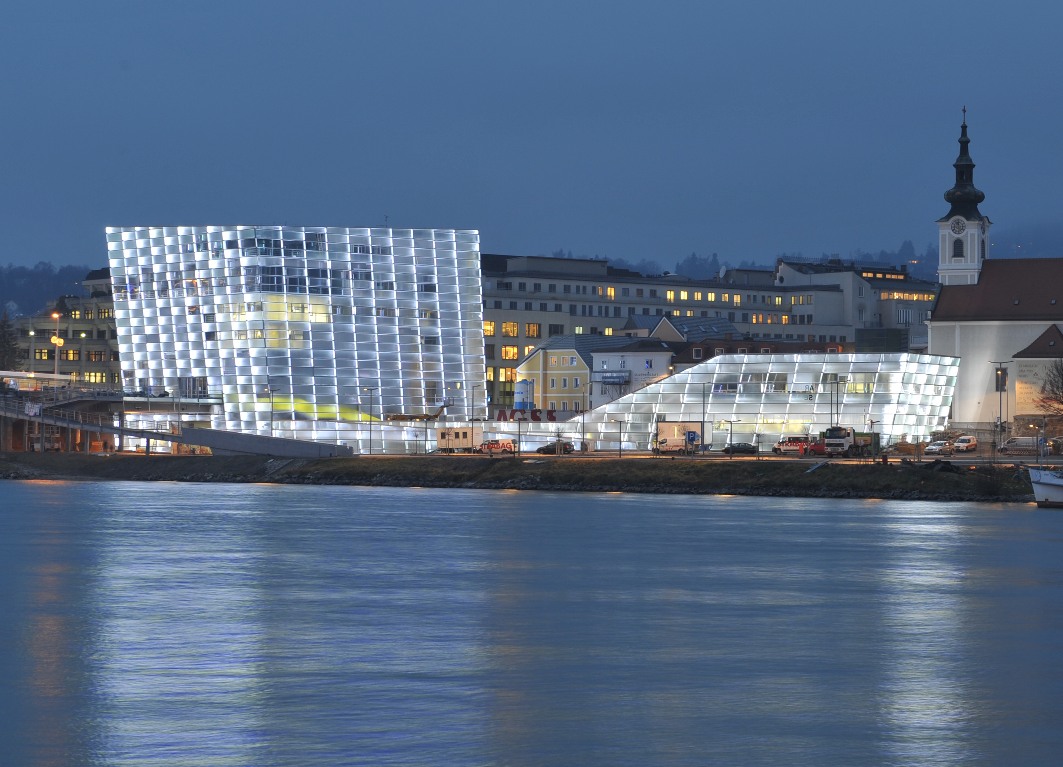
\includegraphics[width=8cm]{exFig.pdf}
% Below the figure, a caption is put, and a label is defined
% to be used for reference to this specific figure.
% Use labels which are very unlikely to be used by
% other contributors; for example, use labels starting
% with the surname of the first author.
\caption{\label{smith:fig1} Caption text \textbf{BELOW} the figure.}
\end{figure}


% In the text, reference to the Figure can be made as follows:
We refer to Figure~\ref{smith:fig1} for a~graphical representation.


%***********************************************************************

% Acknowledgments, if needed:
\acknowledgments{This case study was performed while the first and third author were 
visiting at Biometris at Wageningen University and Research Centre in winter 2014/2015. We are indebted to the group of Prof. Dr. Ruedi Fries, from Technische Universit\"at M\"unchen, for the SNP genotyping of the parental lines, which was funded by the German Federal Ministry of Education and Research (BMBF)  within the AgroClustEr “Synbreed—Synergistic plant and animal breeding” (FKZ:0315528d).}

%***********************************************************************

% References should be placed in the text in author (year) form.
% The list of references should be placed below IN ALPHABETICAL ORDER.
% (Please follow the format of the examples very tightly).

\references
\begin{description}
\item[Diggle, P.J., Liang, K-Y., and Zeger, S.L.] (1994).
     {\it Analysis of Longitudinal Data}.
     Oxford: Clarendon Press.
\item[Green, P.J. and Silverman, B.W.] (1994).
     {\it Nonparametric Regression and Generalized Linear Models}.
     London: Chapman \& Hall.
\item[Henderson, C.R.] (1973).
     Sire evaluation and genetic trends.
     In: {\it Proceedings of the Animal Breeding and Genetics Symposium in
     Honour of Dr.\ L.\ Lush}, Champaign, Illinois, 10\,--\,41.
\item[Lee, Y. and Nelder, J.A.] (1996).
     Hierarchical generalized linear models.
     {\it Journal of the Royal Statistical Society, Series B}, {\bf 58},
      619\,--\,678.
\item[Robinson, G.K.] (1991).
     That BLUP is a good thing: the estimation of random effects (with Discussion).
     {\it Statistical Science}, {\bf 6}, 15\,--\,51.
\end{description}

\end{document}
